\documentclass[10pt]{book}
\usepackage[text=17cm,left=2.5cm,right=2.5cm, headsep=20pt, top=2.5cm, bottom = 2cm,letterpaper,showframe = false]{geometry} %configuración página
\usepackage{latexsym,amsmath,amssymb,amsfonts} %(símbolos de la AMS).7
\parindent = 0cm  %sangria
\usepackage[T1]{fontenc} %acentos en español
\usepackage[spanish]{babel} %español capitulos y secciones
\usepackage{graphicx} %gráficos y figuras.

%---------------FORMATO de letra--------------------%

\usepackage{lmodern} % tipos de letras
\usepackage{titlesec} %formato de títulos
\usepackage[backref=page]{hyperref} %hipervinculos
\usepackage{multicol} %columnas
\usepackage{tcolorbox, empheq} %cajas
\usepackage{enumerate} %indice enumerado
\usepackage{marginnote}%notas en el margen
\tcbuselibrary{skins,breakable,listings,theorems}
\usepackage[Bjornstrup]{fncychap}%diseño de portada de capitulos
\usepackage[all]{xy}%flechas
\counterwithout{footnote}{chapter}
\usepackage{xcolor}
\usepackage[htt]{hyphenat}
%--------------------GRÀFICOS--------------------------

\usepackage{tkz-fct}

%---------------------------------

\titleformat*{\section}{\bfseries\rmfamily}
\titleformat*{\subsection}{\bfseries\rmfamily}
\titleformat*{\subsubsection}{\bfseries\rmfamily}
\titleformat*{\paragraph}{\bfseries\rmfamily}
\titleformat*{\subparagraph}{\bfseries\rmfamily}

%------------------------------------------

\renewcommand{\labelenumi}{\Roman{enumi}.}%primer piso II) enumerate
\renewcommand{\labelenumii}{\arabic{enumii}$)$}%segundo piso 2)
\renewcommand{\labelenumiii}{\alph{enumiii}$)$}%tercer piso a)
\renewcommand{\labelenumiv}{$\bullet$}%cuarto piso (punto)

%----------Formato título de capítulos-------------

\usepackage{titlesec}
\renewcommand{\thechapter}{\arabic{chapter}}
\titleformat{\chapter}[display]
{\titlerule[2pt]
\vspace{4ex}\bfseries\sffamily\huge}
{\filleft\Huge\thechapter}
{2ex}
{\filleft}

\begin{document}

\normalfont
\input xy
\xyoption{all}
\author{\Large Apuntes por FODE}
\title{\small Daniel M. Hausman \\ \vspace{1cm} \large La filosofía de la economía: Una ontología}
\date{}
\pagestyle{empty}
\maketitle
\thispagestyle{empty}
\let\cleardoublepage\clearpage
\tableofcontents								%indice





\begin{document}
    
    %-------------------- wooldridge -------------------------

	%---------- caratula
	    %\begin{titlingpage}

\newcommand\nbvspace[1][3]{\vspace*{\stretch{#1}}}
% allow some slack to avoid under/overfull boxes
\newcommand\nbstretchyspace{\spaceskip0.5em plus 0.25em minus 0.25em}
% To improve spacing on titlepages
\newcommand{\nbtitlestretch}{\spaceskip0.6em}
\pagestyle{empty}

\begin{center}
\bfseries
\nbvspace[1]

\Large Steven Brakman, Harry Garretsen, y Charles van Marrewijk\\
\Huge
{\nbtitlestretch\Huge LA NUEVA INTRODUCCIÓN A LA ECONOMÍA GEOGRÁFICA.}\\
\vspace{.5cm}
\large
\nbvspace[1]

APUNTES\\

\nbvspace[1]
\small POR\\
\Large FODE\\[0.5em]
\footnotesize CHRISTIAN LIMBERT PAREDES AGUILERA\\

\nbvspace[2]

\begin{center}
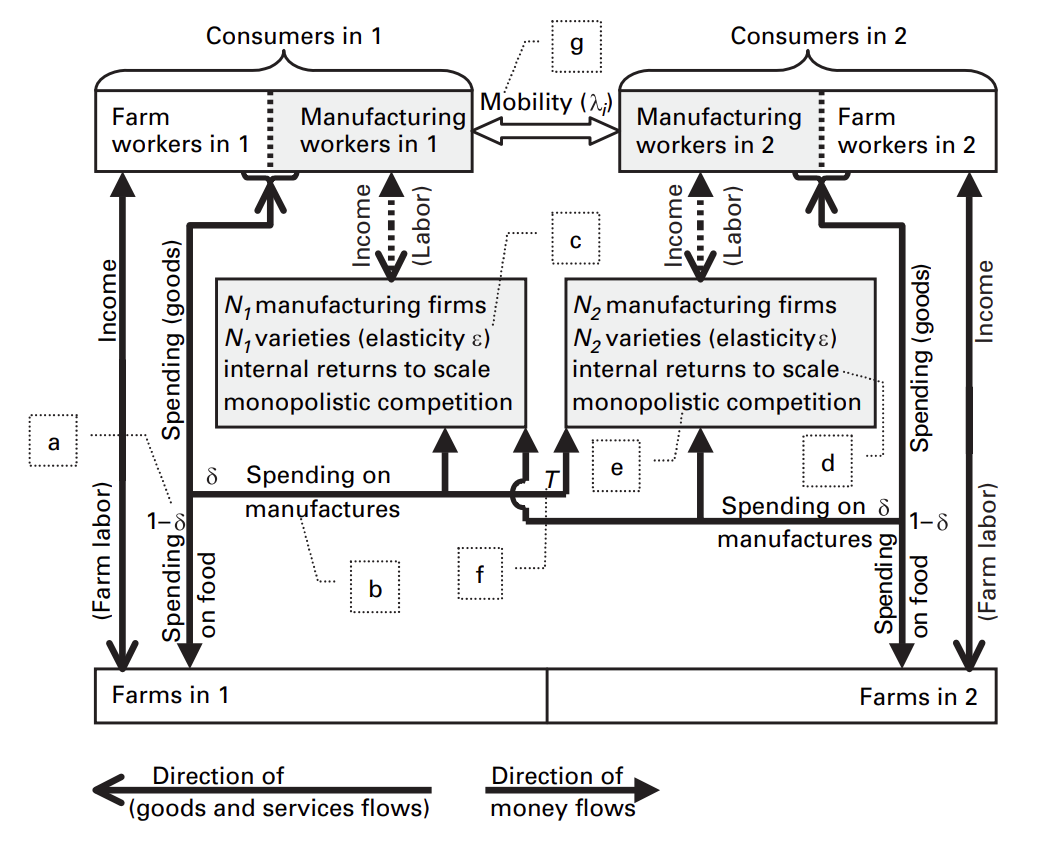
\includegraphics[scale=.3]{./imagen/diag.png}
\end{center}

\nbvspace[3]
\normalsize

LIBRO EN SU SEGUNDA EDICIÓN (Ingles)\\
\large
\nbvspace[1]

\end{center}

\break
\bfseries 

\nbvspace[1]
Título de la obra original:\\
THE NEW INTRODUCTION TO GEOGRAPHICAL ECONOMICS\\
Published in the United States of America by Cambridge University Press, New York\\

\nbvspace[1]

\begin{center}
Sin ninguna revisión de esta obra.\\


\nbvspace[1]
    Propiedad de esta obra:\\ 

    CHRISTIAN LIMBERT PAREDES AGUILERA\\	

    E-mail: soyfode@gmail.com
\end{center}

\nbvspace[1]

Reservados todos los derechos. La reproducción total o parcial de esta obra, por cualquier medio o procedimiento, comprendidos la reprografía y el tratamiento informático, y la distribución de ejemplares de ella mediante alquiler o préstamo públicos, queda rigurosamente prohibida sin la autorización escrita de los titulares del copyright, bajo las sanciones establecidas por las leyes.\\

\center 2022 

\end{titlingpage}


\pagenumbering{roman}

\tableofcontents								%indice

\pagestyle{fancy}
\fancyhead[LE,RO]{\nouppercase{\truncate{0.5\headwidth}{\rightmark}}}
\fancyhead[LO,RE]{\nouppercase{\truncate{0.5\headwidth}{\leftmark}}}



        %---------- Capítulo 2 El modelo de regresión simple
	    %\setcounter{chapter}{1}
\chapter{El modelo de regresión simple}
\section{Definición del modelo de regresión simple}
\begin{equation}
    y = \beta_o + \beta_1x + u.
\end{equation}

\section{Obtención de las estimaciones de mínimos cuadrados ordinarios}

Sea $\left\{(x_i,y_i): i = 1,\ldots,n\right\}$, una muestra aleatoria de tamaño $n$ tomada de la población. Como estos datos provienen de $(2.1)$ para todo $i$ puede escribirse 
\begin{equation}
    y_i = \beta_o + \beta_1x_i + u_i.
\end{equation}

En tanto el intercepto $\beta_0$ aparezca en la ecuación, nada se altera al suponer que el valor promedio de $u$ en la población, es cero. Es decir, $E(u)=0$.\\
El supuesto crucial es que el valor promedio de $u$ no depende del valor de $x$. Este supuesto se expresa como $u$ $E(u\backslash x) = E(u)$. Esta última ecuación indica que el valor promedio de los factores no observables es el mismo en todas las fracciones de la población determinados por los valores de $x$ y que este promedio común es necesariamente igual al promedio al promedio de $u$ en toda la población. Y por lo tanto $u$ es media independiente de $x$. Combinando la independencia de la media con el supuesto de $E(u)=0$ se obtiene el supuesto de media condicional cero, $E(u\backslash x) = 0$\\\\

En la población, $u$ no está correlacionada con $x$. Por tanto, se tiene que el valor esperado de $u$ es cero y que la covarianza entre $x$ y $y$ es cero:
\begin{equation}
    E(u)=0
\end{equation}
 y 

\begin{equation}
    Cov(x,u) = E(xu) =0.
\end{equation}

\textbf{Covarianza.-} Sean $\mu_x = E(X)$ y $\mu_y = E(Y)$ y considere la variable aleatoria $(X-\mu_x)(Y-\mu_y)$. Si $X$ es mayor a su media y $Y$ es mayor a su media, entonces $(X-\mu_x)(Y-\mu_y)>0$. La covarianza entre dos variables aleatorias $X$ y $Y$ llamada algunas veces covarianza poblacional, para hacer énfasis en que se refiere a la relación entre dos variables que describen una población, está definida como el valor esperado del producto $(X-\mu_x)(Y-\mu_y)$: 

\begin{equation}
    Cov(X,Y) = E\left[(X-\mu_x)(Y-\mu_y)\right]
\end{equation}

que también suele denotarse como $\sigma_{XY}.$  \\
Algunas expresiones para útiles para calcular $Cov(X,Y)$ son las siguientes

\begin{equation}
    Cov(X,Y) = E\left[(X-\mu_x)(Y-\mu_y)\right] = E\left[(X-\mu_X)Y\right] = E\left[X(Y-\mu_Y)\right] = E(XY) - \mu_x \mu_y
\end{equation}

De donde se sigue que si $E(X)=0$ o $E(Y)=0$, entonces $Cov(X,Y) = E(XY)$.\\\\

Luego  
\begin{equation}
    E(y - \beta_0 - \beta_1x) = 0
\end{equation}
 
y 

\begin{equation}
    E\left[x(y - \beta_0 -\beta_i x )\right] = 0.
\end{equation}

Como hay que estimar dos parámetros desconocidos, se espera que las dos ecuaciones anteriores puedan servir para obtener buenos estimadores de $\beta_0$ y $\beta_1$. En efecto estas ecuaciones pueden servir para la estimación de estos parámetros.\\\\

Por el método de momentos para la estimación , y las anteriores dos ecuaciones,
\begin{equation}
    n^{-1} \sum\limits_{i=1}^n (y_i - \beta_0 - \beta_1x_i) = 0
\end{equation}
y 
\begin{equation}
    n^{-1} \sum\limits_{i=1}^n x_i(y_i - \beta_0 - \beta_1x_i) = 0
\end{equation}
también llamada \textbf{condiciones de primer orden para los estimadores de MCO}. Luego por la ecuación (2.9) tenemos que 
\begin{equation}
    \overline{y} = \hat{\beta_0} + \hat{\beta_1}\overline{x}.
\end{equation}
donde $\overline{y} = n^{-1}\sum\limits_{i=1}^n y_i$ es el promedio muestral de las $y_i$, y lo mismo ocurre con $\overline{x}$, así, 

\begin{tcolorbox}[colframe=white]
\begin{equation}
    \hat{\beta_0} = \overline{y} - \hat{\beta_1}\overline{x}.
\end{equation}
\end{tcolorbox}
Por último empleando (2.10) y (2.12) para sustituir $\hat{\beta_0}$ se obtiene,
$$\sum_{i=1}^n x_i\left[y_i-(\overline{y}-\hat{\beta_1}\overline{x})-\hat{\beta_1}x_i\right] = 0,$$
de donde, reordenando, tenemos que
$$\sum_{i=1}^n x_i(y_i-\overline{y}) = \hat{\beta_1}\sum_{i=1}^n x_i(x_i-\overline{x}).$$
en consecuencia por las propiedades de la sumatoria, 
$$\sum_{i=1}^n x_i(x_i-\overline{x}) = \sum_{i=1}^n (x_i-\overline{x})^2 \quad y \quad \sum_{i=1}^n x_i(y_i-\overline{y}) = \sum_{i=1}^n (x_i-\overline{x})(y_i-\overline{y})$$\\
ya que $\sum\limits_{i=1}^n (x_i-\overline{x})(y_i-\overline{y})=\sum\limits_{i=1}^n x_i y_i - \overline{y}\sum\limits_{i=1}^n x_i - \overline{x}\sum\limits_{i=1}^n y_i + \overline{y} \overline{x}\sum\limits_{i=1}^n 1 $, luego ya que $\sum\limits_{i=1}^n x_i = n\overline{x}$ entonces $\sum\limits_{i=1}^n x_iy_i - n\overline{yx} - n\overline{xy} + n\overline{xy} = \sum\limits_{i=1}^n x_i(y_i-\overline{y})$
por lo tanto, 
\begin{tcolorbox}[colframe=white]
\begin{equation}
    \hat{\beta_1} = \frac{\sum\limits_{i=1}^n (x_i-\overline{x})(y_i-\overline{y})}{\sum\limits_{i=1}^n (x_i-\overline{x})^2}.
\end{equation}
\end{tcolorbox}
Ésta ecuación no es nada mas que la covarianza muestral en $x$ e $y$ dividida entre la variación muestral de $x$. Esto tiene sentido porque $\beta_1$ es igual a la covarianza poblacional dividida entre la varianza de $x$ cuando $E(u)=0$ y $Cov(x,u) = 0$. Como consecuencia directa se tiene que si en la muestra $x$ e $y$ están correlacionadas positivamente, entonces $\hat{\beta_1}$ es positiva y contrariamente.\\\\
Para todo $\hat{\beta_0}$ y $\hat{\beta_1}$ se define el valor ajustado para $y$ cuando $x=x_i$ como 
\begin{equation}
	\hat{y_i} = \hat{\beta_0} + \hat{\beta_1}x_i.
\end{equation}
Este es el valor que se predice para $y$ cuando $x=x_i$.\\\\
El \textbf{residual} de la observación $i$ es la diferencia entre el verdadero valor $y_i$ y su valor ajustado.\begin{equation} 
    \hat{u} = y_i - \hat{y_i} = y_i - \hat{\beta_0} - \hat{\beta_1}x_i.
\end{equation}
Los residuales no son lo mismo que la ecuación (2.2)\\\\
Supongamos que $\hat{\beta_0}$ y $\hat{\beta_1}$, se eligen de manera que la suma de residuales cuadrados, 
\begin{equation}
    \sum\limits_{i=1}^n \hat{u_i}^2 = \sum\limits_{i=1}^n (y_i - \hat{\beta_0} - \hat{\beta_1}x_i)^2
\end{equation}
sea tan pequeña como sea posible. \\\\

\textbf{Minimización de la suma de los residuos cuadrados.-}
Se mostrará que $\hat{\beta_0}$ y $\hat{\beta_1}$ estimados de MCO minimizan la suma de los residuales cuadrados. Formalmente, el problema es encontrar las soluciones $\hat{\beta_0}$ y $\hat{\beta_1}$ del problema de minimización 
$$\min_{b_0,b_1} \sum_{i=1}^n (y_i-b_0-b_ix_i)^2$$
donde $b_0$ y $b_1$ son argumentos ficticios en el problema de optimización. Para simplificar llámesele a esta función $Q(b_0,b_1)$. Una condición para que $\hat{\beta_0}$ y $\hat{\beta_1}$ sean soluciones del problema de minimización es que las derivadas parciales de $Q(b_0,b_1)$ respecto a $b_0$ y $b_1$ evaluadas en $$\hat{\beta_0},\hat{\beta_1}: \quad \dfrac{\partial Q(\hat{\beta_0},\hat{\beta_1})}{\partial b_0}=0 \qquad y \qquad \dfrac{\partial Q(\hat{\beta_0},\hat{\beta_1})}{\partial b_1}=0$$
Con ayuda de la regla de la cadena del cálculo, estas dos ecuaciones se convierten en,
$$-2\sum_{i=1}^n \hat{u} = -2\sum_{i=1}^n(y_i-\hat{\beta}_0 - \hat{\beta}_1 x_i)=0, \qquad -2\sum_{i=1}^n x_1\hat{u} = -2\sum_{i=1}^n x_i(y_i-\hat{\beta}_0 - \hat{\beta}_1 x_i)=0$$
Una manera de comprobar que se ha minimizado la suma de los residuos cuadrados es expresando, para cualquier $b_0$ y $b_1$,
$$\begin{array}{rcl}
    Q(b_0,b_1)&=&\sum\limits_{i=1}^n \left[y_i-\hat{\beta}_0 - \hat{\beta}_1 + (\hat{\beta}_0 - \hat{\beta}_1 - b_0) + (\hat{\beta}_i - b_1)x_i\right]^2\\\\
	      &=&\sum\limits_{i=1}^n \left[\hat{u}_i + (\hat{\beta}_0 - b_0) + (\hat{\beta}_i - b_1)x_i\right]^2\\\\
	      &=&\sum\limits_{i=1}^n \hat{u}_1^2 + n(\hat{\beta}_0-b_0)^2 + (\hat{\beta}_1-b_1)\sum\limits_{i=1}^n x_i^2 + 2(\hat{\beta}_0-b_0)(\hat{\beta}_1-b_1)\sum\limits_{i=1}^n x_i\\\\
\end{array}$$
Luego ya que el primer termino no depende de $b_0$ ni de $b_1$ entonces,
$$\sum_{i=1}^n \left[(\hat{\beta}_0-b_0)+(\hat{\beta}_1-b_1)x_i\right]^2$$
Dado que ésta es una suma de términos al cuadrado, el menor valor que puede tener es 0. Por lo tanto, tendrá el menor valor posible cuando $b_o=\hat{\beta}_0$ y $b_1=\hat{\beta}_1$.\\\\

Con MCO se podrá obtener insesgamiento, consistencia y otras propiedades estadísticas de una manera relativamente sencilla. Además, como sugiere la motivación en las ecuaciones (2.8) y (2.9)  y como se verá en la sección 2.5, el método de MCO es adecuado para estimar los parámetros que aparecen en la función de la media condicional.\\\\

Una vez que se han determinado las estimaciones por MCO del intercepto y de la pendiente,
se obtiene la \textbf{línea de regresión de MCO o función de regresión muestral (FRM)}:

\begin{tcolorbox}[colframe=white]
    \begin{equation}
	\hat{y} = \hat{\beta}_0 + \hat{\beta}_1 x.
    \end{equation}
\end{tcolorbox}

Donde se entiende que $\hat{\beta}_0$ y $\hat{\beta}_1$ han sido obtenidas empleando las ecuaciones (2.12) y (2.13). La notación $\hat{y}$ que se lee $y \; gorro$ indica los valores predichos por la ecuación (2.17) son estimaciones. \\\\
En la mayoría de los casos, la pendiente estimada, se puede expresar como,
\begin{equation}
    \hat{\beta}_1 = \dfrac{\triangle \hat{y}}{\triangle x}
\end{equation}
es de mayor interés, pues indica la cantidad en la que cambia $\hat{y}$ cuando $x$ se incrementa en una unidad. De manera equivalente,
\begin{equation}
    \hat{y} =  \hat{\beta}_1 \triangle x.
\end{equation}

\section{Propiedades de MCO en cualquier muestra de datos}
El residual de MCO correspondiente a la observación $i$, $\hat{u}_i$, es la diferencia entre $y_i$ y su valor ajustado, como se indica en la ecuación (2.15). Si $\hat{u}_i$ es positivo, la línea predice un valor que subestima al de $y_i$; si $\hat{u}_i$ es negativo, la linea predice un valor en exceso al de $y_i$. Lo ideal para la observación $i$ es cuando $\hat{u}_i = 0$, pero en la mayoría de los casos todos los residuales son distintos de cero. 

\subsection{Propiedades algebraicas de los estadísticos de MCO}
Las estimaciones de $MCO$ y sus correspondientes estadísticos tiene varias propiedades útiles. A continuación se verán las tres más importantes.
\begin{enumerate}[\bfseries 1.]

    \item La suma y por tanto el promedio muestral de los residuales de MCO, es cero. Matemáticamente
	\begin{equation}
	    \sum_{i=1}^n \hat{u}_i = 0.
	\end{equation}

    \item La covarianza muestral entre los regresores y los residuales de MCO es cero. Esto es consecuencia de la condición de primer orden (2.10) que en términos de los residuales puede expresarse como
    	\begin{equation}
	    \sum_{i=1}^n x_i \hat{u}_i = 0.
	\end{equation}

	El promedio muestral de los residuos de MCO, es cero, por lo que el lado izquierdo de la ecuación anterior es proporcional a la covarianza entre las $x_i$ y los $\hat{u}_i$.

    \item El punto $(\overline{x},\overline{y})$ se encuentran siempre sobre la línea de regresión de MCO. En otras palabras, si en la ecuación $\hat{y} = \hat{\beta}_i x + \hat{\beta}_o$ se sustituye $\overline{x}$ por $x$, el valor predicho es $\overline{y}$. Esto es exactamente lo que dice la ecuación $\overline{y} = \hat{\beta}_0 + \hat{\beta}_1 \overline{x}$.\\\\
\end{enumerate}

Sea 
\begin{equation}
    y_i = \hat{y}_i + \hat{u}_i.
\end{equation}
Por la propiedad 1, el promedio de los residuos es cero, equivalentemente, el promedio muestral de los valores ajustados $\hat{y}_i$, es el mismo que el promedio muestral de $y_i$ o $\overline{\hat{y}} = \overline{y}$\\
además por la propiedad 1 y 2  muestra que la covarianza muestral entre $\hat{y}$ y $\hat{u}$ es cero. Entonces podemos ver que a $MCO$  como la descomposición de $y_i$ en dos partes, un valor ajustado y un residual. De los cuales no están correlacionados en la muestra.\\\\

Definamos el \textbf{total de la suma de los cuadrados}\\

\begin{equation}
    SST = \sum\limits_{i=1}^n (y_i - \overline{y})^2
\end{equation}
SST es una medida de la variación total de la muestra en $y_i$; es decir, mide qué tan dispersos están los $y_i$ en la muestra. Si dividimos por $n-1$ obtendremos la varianza muestral de $y$\\\\

luego el \textbf{Suma Explicada de cuadrados}\\

\begin{equation}
    SSE = \sum\limits_{i=1}^n (\hat{y}_i - \overline{y})^2
\end{equation}
SSE mide la variación muestral en $\hat{y}_i$ (donde usamos el hecho de que $\overline{\hat{y}} = \overline{y}$\\\\ 
Y la \textbf{suma de cuadrados residuales (SSR)}

\begin{equation}
    SSR = \sum\limits_{i=1}^n \hat{u}_i^2 
\end{equation}
SSR mide la variación muestral en $\hat{u}_i$\\\\

La variación total en $y$ puede expresarse como la suma de las variaciones explicativas y la variación no explicativa SSR, 
\begin{equation}
	SST = SSE + SSR
\end{equation}
Demostración.-\; 
$$\begin{array}{rcl}
    \sum\limits_{i=1}^n (y_i - \overline{y})^2&=&\sum\limits_{i=1}^n\left[(y_i - \hat{y})+(\hat{y}_i - \overline{y})\right]^2\\\\
					      &=&\sum\limits_{i=1}^n \left[\hat{u}_i + (\hat{y}_i - \overline{y})\right]^2 \\\\
					      &=&\sum\limits_{i=1}^n \hat{u}_i + 2\sum\limits_{i=1}^n\hat{u}(\hat{y}-\overline{y}) + \sum\limits_{i=1}^n (\hat{y}_i - \overline{y})^2\\\\
					      &=&SSR + \sum\limits_{i=1}^n \hat{u}_i (\hat{y}_i - \overline{y}) + SSE\\\\
\end{array}$$
Ahora (2.36) es verdadera si se muestra que 
$$\sum_{i=1}^n \hat{u}_i (\hat{y}_i - \overline{y}) = 0$$
Pero ya se a dicho que la covarianza mueestral entre los residuos y los valores ajustados es vero y esta covarianza es precisamente (2.37) dividida entre $n-1$.\\\\

\subsection{Bondad de ajuste}
Hasta ahora, no tenemos forma de medir qué tan bien la variable explicativa o independiente, $x$, explica la variable dependiente $y$. Para ello dividimos (2.26) por $SST$ para que nos quede $1=SSE/SST + SSR/SST$. EL r cuadrado de la regresión, a veces es llamado \textbf{coeficiente de determinación} y es definido por,
\begin{equation}
	R^2 = SSE/SST = 1 - SSE/SST
\end{equation}

$R^2$ es el razón de la variación explicada en comparación con la variación total. Por tanto, se interpreta como la fracción de la variación muestral en $y$ que se explica por $x$. Usualmente el resultado es multiplicado por $100$ para que nos de en un porcentaje.\\
\textbf{Si todos los puntos de datos se encuentran en la misma línea, MCO proporciona un ajuste perfecto a los datos. En este caso, $R_2 = 1$. Un valor de $R_2$ que es casi igual a cero indica un mal ajuste de la línea MCO}.\\
De hecho, se puede demostrar que $R_2$ es igual al cuadrado del coeficiente de correlación muestral entre $y_i$ y $hat{y}^i$.\\\\
Vale la pena enfatizar ahora que un R cuadrado aparentemente bajo no significa necesariamente que una ecuación de regresión MCO sea inútil. Tenga en cuenta que el uso de R-cuadrado como principal indicador del éxito de un análisis econométrico puede generar problemas.\\\\

\section{Valores esperados y varianzas de los estimadores de MCO}




    %-------------------- dougherty -------------------------

	%----------caratula
	    %\begin{titlingpage}

\newcommand\nbvspace[1][3]{\vspace*{\stretch{#1}}}
% allow some slack to avoid under/overfull boxes
\newcommand\nbstretchyspace{\spaceskip0.5em plus 0.25em minus 0.25em}
% To improve spacing on titlepages
\newcommand{\nbtitlestretch}{\spaceskip0.6em}
\pagestyle{empty}

\begin{center}
\bfseries
\nbvspace[1]

\Large Steven Brakman, Harry Garretsen, y Charles van Marrewijk\\
\Huge
{\nbtitlestretch\Huge LA NUEVA INTRODUCCIÓN A LA ECONOMÍA GEOGRÁFICA.}\\
\vspace{.5cm}
\large
\nbvspace[1]

APUNTES\\

\nbvspace[1]
\small POR\\
\Large FODE\\[0.5em]
\footnotesize CHRISTIAN LIMBERT PAREDES AGUILERA\\

\nbvspace[2]

\begin{center}
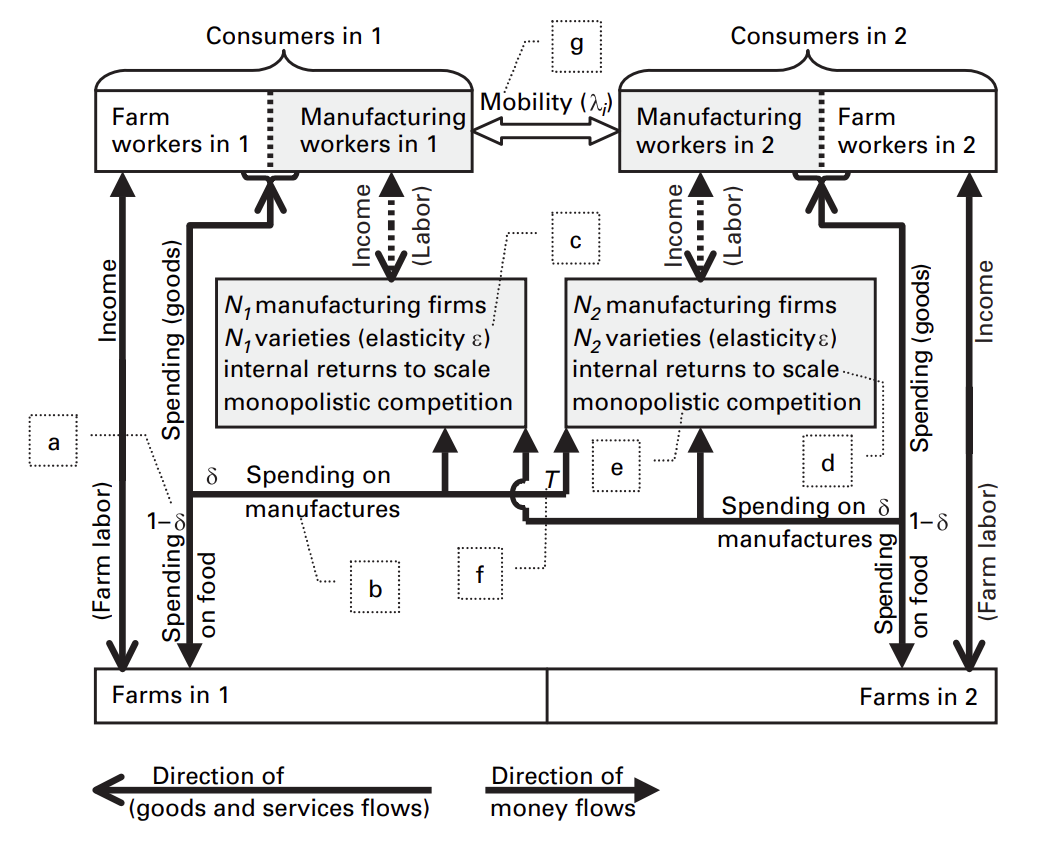
\includegraphics[scale=.3]{./imagen/diag.png}
\end{center}

\nbvspace[3]
\normalsize

LIBRO EN SU SEGUNDA EDICIÓN (Ingles)\\
\large
\nbvspace[1]

\end{center}

\break
\bfseries 

\nbvspace[1]
Título de la obra original:\\
THE NEW INTRODUCTION TO GEOGRAPHICAL ECONOMICS\\
Published in the United States of America by Cambridge University Press, New York\\

\nbvspace[1]

\begin{center}
Sin ninguna revisión de esta obra.\\


\nbvspace[1]
    Propiedad de esta obra:\\ 

    CHRISTIAN LIMBERT PAREDES AGUILERA\\	

    E-mail: soyfode@gmail.com
\end{center}

\nbvspace[1]

Reservados todos los derechos. La reproducción total o parcial de esta obra, por cualquier medio o procedimiento, comprendidos la reprografía y el tratamiento informático, y la distribución de ejemplares de ella mediante alquiler o préstamo públicos, queda rigurosamente prohibida sin la autorización escrita de los titulares del copyright, bajo las sanciones establecidas por las leyes.\\

\center 2022 

\end{titlingpage}


\pagenumbering{roman}

\tableofcontents								%indice

\pagestyle{fancy}
\fancyhead[LE,RO]{\nouppercase{\truncate{0.5\headwidth}{\rightmark}}}
\fancyhead[LO,RE]{\nouppercase{\truncate{0.5\headwidth}{\leftmark}}}



	%----------review
	    %\chapter{Review}

\section{Exercises}


	%---------- Regresión lineal
	    %\chapter{Análisis de Regresión simple}
\begin{multicols}{2}
%-------------------- ecuación 1.1
\begin{tcolorbox}[colframe = white]
    \begin{equation}
	Y_i = \beta_0 + \beta_1 X_i + u_i 
    \end{equation}
\end{tcolorbox}

\textbf{Nota}.- $u$ en algunas veces es descrito como ruido.\\\\

\setcounter{section}{1}
\section{Regresión de mínimos cuadrados con una variable explicativa}
%-------------------- ecuación 1.2
\begin{tcolorbox}[colframe = white]
    \begin{equation}
	\hat{Y}_i = b_1 + b_2 X_i 
    \end{equation}
\end{tcolorbox}
\textbf{El primer paso}.- es definir que se conoce como residuo de cada observación. El residuo es la diferencia entre el valor real de $Y$ en cualquier observación y el valor ajustado dado por la línea de regresión.

%-------------------- ecuación 1.3
\begin{tcolorbox}[colframe = white]
    \begin{equation}
	e_i = Y_i - \hat{Y}_i
    \end{equation}
\end{tcolorbox}

Substituyendo (1.2) en (1.3) obtenemos:

%-------------------- ecuación 1.4
\begin{tcolorbox}[colframe = white]
    \begin{equation}
	e_i = Y_i - b_1 - b_2 X_i
    \end{equation}
\end{tcolorbox}
y por lo tanto el residuo en cada observación depende de la elección de $b_1$ y $b_2$. Obviamente, deseamos ajustar la recta de regresión, es decir, elegir $b_1$ y $b_2$, de tal manera que los residuos sean lo más pequeños posible. La mejor manera de hacer esto posible es es minimizando $RSS$ el residuo de las sumas cuadradas 

%-------------------- ecuación 1.5
\begin{tcolorbox}[colframe = white]
    \begin{equation}
	RSS = e_1^2 + e_2^2 + ... + e_n^2
    \end{equation}
\end{tcolorbox}

\section{Calculando los coeficientes de regresión}
Supondremos que el verdadero modelo es
%-------------------- ecuación 1.6
\begin{tcolorbox}[colframe = white]
    \begin{equation}
	Y_i = \beta_0 + \beta_1 X_i + u_i 
    \end{equation}
\end{tcolorbox}
y supondremos que los coeficientes $b_1$ y $b_2$ de la ecuación 
%-------------------- ecuación 1.7
\begin{tcolorbox}[colframe = white]
    \begin{equation}
	\hat{Y}_i = b_1 + b_2 X_i
    \end{equation}
\end{tcolorbox}
La tabla siguiente nos hará entender mejor el asunto
$$\begin{array}{cccc}
    X&Y&\hat{Y}&e\\\\
    \hline\\
     1&3&b_1+b_2&e_1 = 3-b_1-b_2\\\\
     2&5&b_1+2b_2&e_2 = 5-b_1-2b_2\\\\
     3&6&b_1+3b_2&e_3 = 6-b_1-3b_2
\end{array}$$
Por lo tanto aplicando (1.5)
%-------------------- ecuación 1.8

\begin{equation}
\begin{tabular}{rcl}
    RSS & = & $(3-b_1-b_2)^2 + (5-b_1-2b_2)^2 + (6-b_1-3b_2)^2$\\\\
	& = & $9+b_1^2 + b_2^2 - 6b_1 - 6b_2 + 2b_1b_2 + 25 + b_1^2 + 4b_2^2 - 10b_1$ \\\\
	&  & $- 20b_2 + 4b_1b_2 + 36 +b_1^2 + 9b_2^2 - 12b_1 - 36b_2 + 6b_1b_2 $\\\\
	& = &  $70 + 3b_1^2 + 14b_2^2 -28b_1 -62b_2 +12b_1b_2$\\
\end{tabular}
\end{equation}


Ahora queremos elegir $b_1$ y $b_2$ para minimizar $RSS$. Para ello usamos al calculo para definir estos valores y pueda satisfacer las condiciones de primer orden
%-------------------- ecuación 1.9
\begin{tcolorbox}[colframe = white]
\begin{equation}
    \dfrac{\partial RSS}{\partial b_1} = 0 \qquad y \qquad \dfrac{\partial RSS}{\partial b_2} = 0
\end{equation}
\end{tcolorbox}
Tomando diferencias parciales,
%-------------------- ecuación 1.10
\begin{equation}
    \dfrac{\partial RSS}{\partial b_1} = 6b_1 + 12b_2 -28 
\end{equation}
\vspace{.5cm}
%-------------------- ecuación 1.11
\begin{equation}
    \dfrac{\partial RSS}{\partial b_2} = 28b_2 + 12b_1 - 62 
\end{equation}
así tenemos que
%-------------------- ecuación 1.12
\begin{equation}
    3b_1 + 6b_2 - 14 = 0
\end{equation}
y
%-------------------- ecuación 1.13
\begin{equation}
    6b_1 +14b_2 - 31 = 0
\end{equation}
Resolviendo estas dos ecuaciones, obtenemos que $b_1=1.67$ y $b_2=1.5$ por lo tanto la regresión estará dada por
%-------------------- ecuación 1.14
\begin{equation}
    Y_i = 1.67 + 1.5 X_i
\end{equation}
\vspace{.5cm}

\subsection{Regresión de mínimos cuadrados con una variable explicativa: Caso general}
Supongamos que hay $n$ observaciones para dos variables $X$ y $Y$ y este depende de $X$, ajustaremos la ecuación
%-------------------- ecuación 1.15
\begin{tcolorbox}[colframe = white]
    \begin{equation}
	\hat{Y}_i = b_1 + b_2 X_i,
    \end{equation}
\end{tcolorbox}
El ajustado de la variable dependiente en $i$ observaciones, $\hat{Y}_i$, será $(b_1+b_2X_i)$ y el residuo $e_i$ será $(Y_i -b_1 - b_2X_i)$, entonces para minimizar el residuo de los mínimos cuadrados $RSS$, se tendrá la ecuación,
%-------------------- ecuación 1.16
\begin{tcolorbox}[colframe = white]
    \begin{equation}
	RSS = e_1^2 + \ldots + e_n^2 = \sum_{i=1}^{n} e_i^2
    \end{equation}
\end{tcolorbox}

Sabremos que encontramos el $RSS$ minimizado cuando 
%-------------------- ecuación 1.17
\begin{tcolorbox}[colframe = white]
    \begin{equation}
	b_2 = \dfrac{\sum\limits_{i=1}^n \left(X_i-\overline{X}\right)\left(Y_i - \overline{Y}\right)}{\sum\limits_{i=1}^n \left(X_i - \overline{X}\right)^2}
    \end{equation}
\end{tcolorbox}

y
%-------------------- ecuación 1.18
\begin{equation}
    b_1 = \overline{Y} - b_2 \overline{X}
\end{equation}

Para demostrar comenzaremos expresando el cuadrado del residual en la observación $i$ en términos de $b_1, b_2$ y los datos de $X$ e $Y$:
%-------------------- ecuación 1.19
\begin{equation}
    \begin{tabular}{rcl}
	$e_i^2$ &=& $\left(Y_i - \hat{Y_i}\right)^2$\\\\ 
	      &=& $\left(Y_i - b_i - b_2 X_i\right)^2$ \\\\
	      &=& $Y_i^2 + b_i^2 b_2^2X_i^2 - 2b_iY_i - 2b_2X_iY_i + 2b_i b_2X_i$\\\\
    \end{tabular}
\end{equation}
Sumando sobre todas las $n$ observaciones, podemos escribir $RSS$ como sigue,\\
%-------------------- ecuación 1.20
\begin{equation}
    \begin{tabular}{rcl}
	$RSS$&=&$\left(Y_i - b_i -b_2X-i\right)^2 + \ldots + \left(Y_n - b_1 - b_2X_n\right)^2$\\\\
	     &=&$Y_i^2 + b_i^2 + b_2^2X_i^2 - 2b_iY_i -2b_2X_iY_i + 2b_ib_2X_i$\\\\
	     &=&$\ldots$\\\\
	     &=&$Y_n^2 + b_i^2 + b_2^2X_n^2 - 2b_iY_n - 2b_2X_nY_n + 2b_1b_2 X_n$\\\\
	     &=&$\sum\limits_{i=1}^n Y_i^2 + nb_1^2 + b_2^2\sum\limits_{i=1}^n X_1^2 - 2b_1\sum\limits_{i=1}^n Y_i $\\\\
	     &&$- 2b_2 \sum\limits_{i=1}^n X_iY_i + 2b_i b_2 \sum\limits_{i=1}^n X_i$\\\\
    \end{tabular}
\end{equation}
Luego la condición de primer orden para minimizar, $\partial RSS / \partial b_i = 0$ y $\partial RSS / \partial b_2 = 0$ esta dado por las siguientes ecuaciones,
%-------------------- ecuación 1.21
\begin{tcolorbox}[colframe = white]
    \begin{equation}
	2nb_1 - 2\sum\limits_{i=1}^n Y_i + 2b_2\sum\limits_{i=1}^n X_i = 0
    \end{equation}
\end{tcolorbox}
%-------------------- ecuación 1.22
\begin{tcolorbox}[colframe = white]
    \begin{equation}
	2b_2\sum\limits_{i=1}^n X_i^2 + 2\sum\limits_{i=1}^n X_iY_i + 2b_1\sum\limits_{i=1}^n X_i = 0
    \end{equation}
\end{tcolorbox}

Notemos que (1.21) nos permite escribir $b_1$ en términos de $\overline{Y}$, $\overline{X}$ y el aún desconocido $b_2$. Sea $\overline{X}=\dfrac{1}{n}\sum X_i$ y $\overline{Y} = \dfrac{1}{n}\sum Y_i$ podemos reescribirlo como,
%-------------------- ecuación 1.23
\begin{equation}
    2nb_1 - 2n\overline{Y} + 2b_2n\overline{X} = 0
\end{equation}
y por lo tanto,\\
%-------------------- ecuación 1.24
\begin{tcolorbox}[colframe = white]
    \begin{equation}
	b_1 = \overline{Y} - b_2\overline{X}
    \end{equation}
\end{tcolorbox}
Así sustituyendo por $b_i$ en (1.22) y notanto que $\sum X_i = n\overline{X}$ obtenemos
%-------------------- ecuación 1.25
\begin{equation}
    2b_2 \sum\limits_{i=1}^n X_i^2 + 2\sum\limits_{i=1}^n X_iY_i + 2\left(\overline{Y} - b_2 \overline{X}\right) n\overline{X} = 0
\end{equation}
%-------------------- ecuación 1.26
\begin{equation}
    2b_2\left(\sum\limits_{i=1}^n X_i^2 -n\overline{X}^2 \right) = 2\sum\limits_{i=1}^n X_i Y_i - 2n\overline{X}\overline{Y}
\end{equation}
%-------------------- ecuación 1.27
\begin{tcolorbox}[colframe = white]
    \begin{equation}
	b_2 = \dfrac{\sum\limits_{i=1}^n X_iY_i - n\overline{X}}{2\sum\limits_{i=1}^n X_i^2 - n\overline{X}}
    \end{equation}
\end{tcolorbox}

alternativamente podemos escribir como sigue,\\
%-------------------- ecuación 1.28
\begin{tcolorbox}[colframe = white]
    \begin{equation}
	b_2 = \dfrac{\sum\limits_{i=1}^n \left(X_i - \overline{X}\right) \left(Y_i - \overline{Y}\right)}{\sum\limits_{i=1}^n \left( X_i - \overline{X}\right)^2}
    \end{equation}
\end{tcolorbox}
Lo demostramos de la siguiente manera,\\
%-------------------- ecuación 1.29
\begin{equation}
    \begin{tabular}{rcl}
	&&$\sum\limits_{i=1}^n \left(X_i - \overline{X}\right) \left(Y_i - \overline{Y}\right)$\\\\
	&=&$\sum\limits_{i=1}^n X_iY_i - \sum\limits_{i=1}^n X_i \overline{Y} - \sum\limits_{i=1}^n \overline{X}Y_i + \sum\limits_{i=1}^n \overline{X} \overline{Y}$\\\\
	&=&$\sum\limits_{i=1}^n X_iY_i - \overline{Y}\sum\limits_{i=1}^n X_i - \overline{X}\sum\limits_{i=1}^nY_i + n\overline{XY}$\\\\
	&=&$\sum\limits_{i=1}^n X_iY_i - \overline{Y}\left(n\overline{X}\right) - \overline{X}\left(n\overline{Y}\right)+n\overline{XY}$\\\\
	&=&$\sum\limits_{i=1}^n X_iY_i -n\overline{XY}.$\\\\
    \end{tabular}
\end{equation}
Análogamente podemos demostrar para, \\
%-------------------- ecuación 1.30
\begin{equation}
    \sum\limits_{i=1}^n X_i^2 - n\overline{X}^2 = \sum\limits_{i=1}^n \left(X_i - \overline{X}\right)^2 
\end{equation}
Por último sustituimos $b_2$ en (1.24)\\\\

\subsection{Dos descomposiciones de la variable dependiente}
La primera descomposición se relaciona con el proceso mediante el cual se generan los valores de $Y$:
%-------------------- ecuación 1.31
\begin{equation}
	Y_i = \beta_i + \beta_2X_i + u_i 
\end{equation}

$Y_i$ es generado como la suma de dos componentes, el no estocástico componente $\beta_i + \beta_2 X_i$ y el termino de perturbación $u_i$. Usaremos esto en el análisis de las propiedades de los estimadores de la regresión. En la figura se tiene que $QT$ es el no estocástico componente de $Y$ y $PQ$ es el termino de perturbación.

\begin{center}
    \begin{tikzpicture}[scale=.8,draw opacity = 0.6]
	% abscisa y ordenada
	\tkzInit[xmax= 10,xmin=0,ymax=7,ymin=0]
	\tiny\tkzLabelXY[opacity=0,step=1, orig=false]
	% etiqueta x, f(x)
	\tkzDrawX[opacity=0.6,label=X,right=0.3]
	\tkzDrawY[opacity=0.6,label=Y,below = -0.6]
	%dominio y función
	\draw [domain=0:7,thick] plot(\x,{1/3*\x + 2})node[right]{$\hat{Y} = b_i + b_2X$};
	\draw [domain=0:8,dashed] plot(\x,{2/3*\x + .5})node[right]{$Y = \beta_i + \beta_2X$};
	\draw(0,0.5)node[left]{$\beta_1$};
	\draw(0,2)node[left]{$b_1$};
	\draw[<->](3,0)node[below]{$X_i$}--(3,2.3)node[above right]{$Q$};
	\draw[<->](3,2.7)--(3,4)node[above right]{$P$};
	\filldraw[black] (3,4.2) circle (2pt);
	\filldraw[black] (3,2.5) circle (2pt);
	\draw(3,1.1)node[right]{$\beta_i +\beta_2 X_i$};
	\draw(3,3.4)node[left]{$u_i$};
	\draw(3,0.2)node[right]{$T$};
    \end{tikzpicture}
\end{center}
La otra descomposición se relaciona con la línea de regresión:
\begin{equation}
    Y_i = \hat{Y}_i + e_i = b_i + b_2X_i + e_i 
\end{equation}
donde RT es el valor ajustado y PR es el residuo.

%-------------------- ecuación 1.32

\begin{center}
    \begin{tikzpicture}[scale=.8,draw opacity = 0.6]
	% abscisa y ordenada
	\tkzInit[xmax= 10,xmin=0,ymax=7,ymin=0]
	\tiny\tkzLabelXY[opacity=0,step=1, orig=false]
	% etiqueta x, f(x)
	\tkzDrawX[opacity=0.6,label=X,right=0.3]
	\tkzDrawY[opacity=0.6,label=Y,below = -0.6]
	%dominio y función
	\draw [domain=0:7,thick] plot(\x,{1/3*\x + 2})node[right]{$\hat{Y} = b_i + b_2X$};
	\draw [domain=0:8,dashed] plot(\x,{2/3*\x + .5})node[right]{$Y = \beta_i + \beta_2X$};
	\draw(0,0.5)node[left]{$\beta_1$};
	\draw(0,2)node[left]{$b_1$};
	\draw[<->](3,0)node[below]{$X_i$}--(3,2.75)node[above right]{$R$};
	\draw[<->](3,3.2)--(3,4)node[above right]{$P$};
	\filldraw[black] (3,4.2) circle (2pt);
	\filldraw[black] (3,3) circle (2pt);
	\draw(3,1.1)node[right]{$b_i +b_2 X_i$};
	\draw(3,3.6)node[left]{$e_i$};
	\draw(3,0.2)node[right]{$T$};
    \end{tikzpicture}
\end{center}

\section{Ejercicios}
\begin{enumerate}[\bfseries 1.1]

    %---------- ejercicio 1.1
    \item Supongase que la recta ajustada es $\hat{Y}=b_1+b_1X$ con $b_1$ y $b_2$ definida como las ecuaciones (1.24) y $(1.28)$. Demostrar que la recta ajustada debe pasar a través del punto $\lbrace\overline{X},\overline{Y}\rbrace$ que representa la media de las observaciones en la muestra.\\\\
	Demostración.-\; Sea $X=\overline{X}$ entonces, $\hat{Y} = b_1 + b_2\overline{X}$ luego por (1.24) se tiene que,
	$$\hat{Y} = \overline{Y} - b_2\overline{X} + b_2\overline{X}$$
	de donde,
	$$\overline{Y} = \hat{Y}$$
	Por lo tanto la recta ajustada pasa por el punto $(\overline{X},\overline{Y})$.\\\\

    %---------- ejercicio 1.2
    \item Usando la ecuación normal (1.21) y $(1.22)$, muestre que $b_1$ esta definido, pero $b_2$ no lo está, si $X_i = 0$ para todo $i$. Dar una explicación intuitiva de este resultado.\\\\
	Demostración.-\; Sabiendo que 
	$$2nb_1 - 2\sum\limits_{i=1}^n Y_i + 2b_2\sum\limits_{i=1}^n X_i = 0$$
	$$y$$
	$$2b_2\sum\limits_{i=1}^n X_i^2 + 2\sum\limits_{i=1}^n X_iY_i + 2b_1\sum\limits_{i=1}^n X_i = 0$$\\
	Si $X_i = 0, \forall i$  en (1.21) entonces,\\
	$$b_1 = \dfrac{2\sum\limits_{i=1}^n Y_i}{2n}$$\\
	de donde demostramos que $b_1$ está definida. Y no así $b_2$, ya que si remplazamos $X_i=0\; \forall i$ en (1.22) todas las sumatorias serán $0$.\\\\

    %---------- ejercicio 1.3
    \item Demostrar a partir de los primeros principios que el estimador de mínimos cuadrados de $\beta_i$ en el modelo primitivo donde $Y$ consiste simplemente en una constante más un término de perturbación,
	$$Y_i = \beta_i + u_i$$
	es $b_i = \overline{Y}$\\\\
	Demostración.-\; 
 

\end{enumerate}

\end{multicols}



    %-------------------- Diplomado -------------------------
	

	%----------Apuntes
	%\documentclass[10pt]{book}
\usepackage[text=17cm,left=2.5cm,right=2.5cm, headsep=20pt, top=2.5cm, bottom = 2cm,letterpaper,showframe = false]{geometry} %configuración página
\usepackage{latexsym,amsmath,amssymb,amsfonts} %(símbolos de la AMS).7
\parindent = 0cm  %sangria
\usepackage[T1]{fontenc} %acentos en español
\usepackage[spanish]{babel} %español capitulos y secciones
\usepackage{graphicx} %gráficos y figuras.

%---------------FORMATO de letra--------------------%

\usepackage{lmodern} % tipos de letras
\usepackage{titlesec} %formato de títulos
\usepackage[backref=page]{hyperref} %hipervinculos
\usepackage{multicol} %columnas
\usepackage{tcolorbox, empheq} %cajas
\usepackage{enumerate} %indice enumerado
\usepackage{marginnote}%notas en el margen
\tcbuselibrary{skins,breakable,listings,theorems}
\usepackage[Bjornstrup]{fncychap}%diseño de portada de capitulos
\usepackage[all]{xy}%flechas
\counterwithout{footnote}{chapter}
\usepackage{xcolor}
\usepackage[htt]{hyphenat}
%--------------------GRÀFICOS--------------------------

\usepackage{tkz-fct}

%---------------------------------

\titleformat*{\section}{\bfseries\rmfamily}
\titleformat*{\subsection}{\bfseries\rmfamily}
\titleformat*{\subsubsection}{\bfseries\rmfamily}
\titleformat*{\paragraph}{\bfseries\rmfamily}
\titleformat*{\subparagraph}{\bfseries\rmfamily}

%------------------------------------------

\renewcommand{\labelenumi}{\Roman{enumi}.}%primer piso II) enumerate
\renewcommand{\labelenumii}{\arabic{enumii}$)$}%segundo piso 2)
\renewcommand{\labelenumiii}{\alph{enumiii}$)$}%tercer piso a)
\renewcommand{\labelenumiv}{$\bullet$}%cuarto piso (punto)

%----------Formato título de capítulos-------------

\usepackage{titlesec}
\renewcommand{\thechapter}{\arabic{chapter}}
\titleformat{\chapter}[display]
{\titlerule[2pt]
\vspace{4ex}\bfseries\sffamily\huge}
{\filleft\Huge\thechapter}
{2ex}
{\filleft}

\begin{document}

\normalfont
\input xy
\xyoption{all}
\author{\Large Apuntes por FODE}
\title{\small Daniel M. Hausman \\ \vspace{1cm} \large La filosofía de la economía: Una ontología}
\date{}
\pagestyle{empty}
\maketitle
\thispagestyle{empty}
\let\cleardoublepage\clearpage
\tableofcontents								%indice





\begin{document}
    
    %----------caratula
    %\begin{titlingpage}

\newcommand\nbvspace[1][3]{\vspace*{\stretch{#1}}}
% allow some slack to avoid under/overfull boxes
\newcommand\nbstretchyspace{\spaceskip0.5em plus 0.25em minus 0.25em}
% To improve spacing on titlepages
\newcommand{\nbtitlestretch}{\spaceskip0.6em}
\pagestyle{empty}

\begin{center}
\bfseries
\nbvspace[1]

\Large Steven Brakman, Harry Garretsen, y Charles van Marrewijk\\
\Huge
{\nbtitlestretch\Huge LA NUEVA INTRODUCCIÓN A LA ECONOMÍA GEOGRÁFICA.}\\
\vspace{.5cm}
\large
\nbvspace[1]

APUNTES\\

\nbvspace[1]
\small POR\\
\Large FODE\\[0.5em]
\footnotesize CHRISTIAN LIMBERT PAREDES AGUILERA\\

\nbvspace[2]

\begin{center}
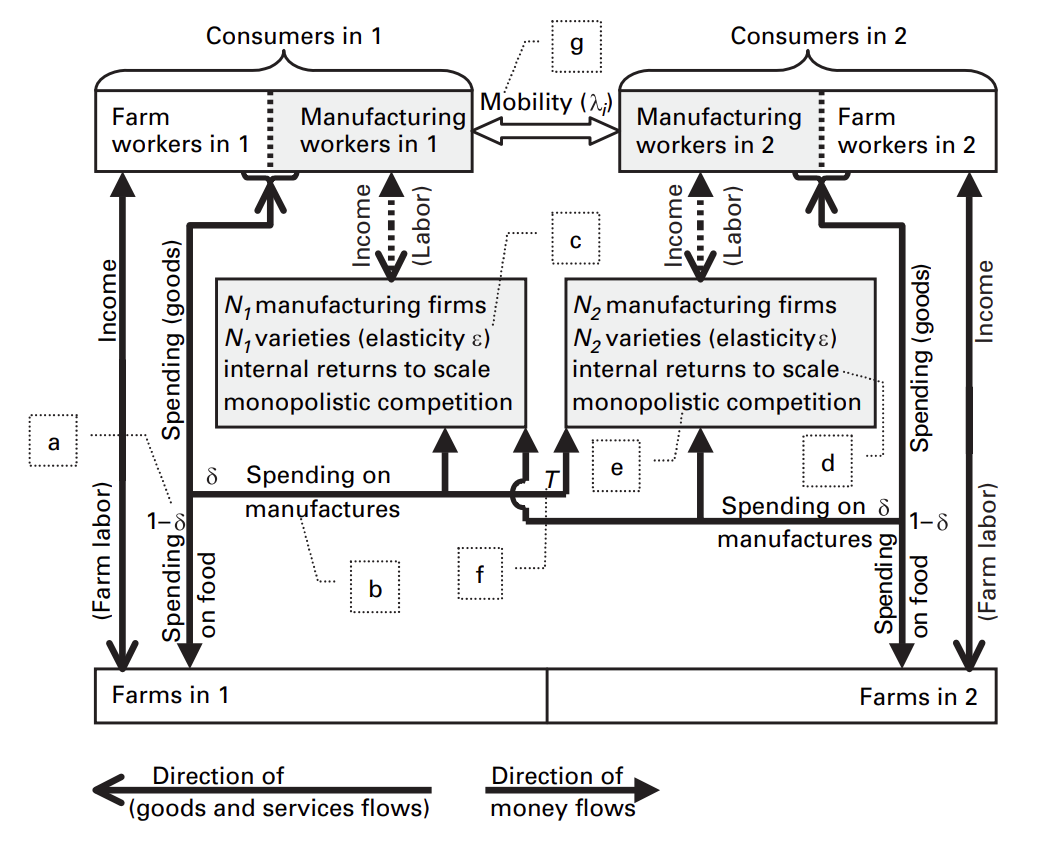
\includegraphics[scale=.3]{./imagen/diag.png}
\end{center}

\nbvspace[3]
\normalsize

LIBRO EN SU SEGUNDA EDICIÓN (Ingles)\\
\large
\nbvspace[1]

\end{center}

\break
\bfseries 

\nbvspace[1]
Título de la obra original:\\
THE NEW INTRODUCTION TO GEOGRAPHICAL ECONOMICS\\
Published in the United States of America by Cambridge University Press, New York\\

\nbvspace[1]

\begin{center}
Sin ninguna revisión de esta obra.\\


\nbvspace[1]
    Propiedad de esta obra:\\ 

    CHRISTIAN LIMBERT PAREDES AGUILERA\\	

    E-mail: soyfode@gmail.com
\end{center}

\nbvspace[1]

Reservados todos los derechos. La reproducción total o parcial de esta obra, por cualquier medio o procedimiento, comprendidos la reprografía y el tratamiento informático, y la distribución de ejemplares de ella mediante alquiler o préstamo públicos, queda rigurosamente prohibida sin la autorización escrita de los titulares del copyright, bajo las sanciones establecidas por las leyes.\\

\center 2022 

\end{titlingpage}


\pagenumbering{roman}

\tableofcontents								%indice

\pagestyle{fancy}
\fancyhead[LE,RO]{\nouppercase{\truncate{0.5\headwidth}{\rightmark}}}
\fancyhead[LO,RE]{\nouppercase{\truncate{0.5\headwidth}{\leftmark}}}



    %---------- Análisis de decisiones económicas y mercados
    %\chapter{Análisis de decisiones económicas y mercados}

\begin{multicols}{2}

\begin{itemize}
    \item Para criticar se debe conocer.
\end{itemize}

\section*{¿Qué preguntas puede abordar la teoría económica?.}

\begin{itemize}
    \item A la economía se le exige a más que otras ciencias. 
    \item ¿El objetivo de la ciencia en predecir?.
    \item El propósito de la ciencia es crear conocimiento donde se crea mundos abstractos.
\end{itemize}

    \subsection*{Objetivos de la economía}

    \begin{itemize}
	\item Entender el mundo real y,
	\item crear un lenguaje para poder discutir.
    \end{itemize}

    \subsection*{Métodos de investigación}
    \begin{itemize}
	\item Las ciencias físicas son mas fáciles que las ciencias económicas. Que sería si los electrones podrían pensar.
	\item Utilizamos el método inductivo.
    \end{itemize}

    \subsection*{¿Cual es el punto de partida para crear mundos abstractos?}
    Las llamamos las tres almas de Smith.
    \begin{enumerate}[1.]
	\item Estudiamos el comportamiento individual de los agentes.
	\item Un grupo es más que la suma de los individuos.
	\item Análisis de instituciones.
    \end{enumerate}
    \textbf{Se partirá del análisis individual}

    \subsection*{Los fundamentos de la escuela neoclásica}

    \begin{itemize}
	\item Se estudia ésta escuela porque es la mas exitosa hasta el momento.
	\item Se tiene tres características para poder ser identificado como neoclásico.
	\begin{enumerate}[1.]
	    \item Ser reduccionistas. Empezamos a analizar a los individuos.
	    \item ¿Que les motiva para tomar acciones?, los agentes deben ser racionales. 
	    \item Tener una noción de equilibro.
	\end{enumerate}
	\item No hay nada peor que estar adoctrinados y no saber lo que creemos.
	\item \textbf{Los economistas estudian decisiones, identificando factores que afectan esas decisiones y el resultado de la interacción de decisiones.}
    \end{itemize}




\end{multicols}


    %---------- Análisis de coyuntura económica (economistas)
    %\chapter{Análisis de coyuntura económica y crecimiento (Economistas)}


    %---------- Análisis de coyuntura económica (no-economistas)
    %\part{Análisis de coyuntura económica (No economistas)}




    %----------Métodos cuantitativos (Estadística)
    %\part{Métodos cuantitativos (Estadística)}

\chapter{Introducción}
\begin{itemize}
    \item La estadística comienza con un objetivo, luego por un estudio estadístico para luego crear conocimiento.
    \item Debemos elegir una población para poder sacar conclusiones.
    \item Se debe tener datos primarios, es decir datos que no existen y datos secundarios que se publican en instituciones publicas o privadas.
\end{itemize}


    %---------- Métodos cuantitativos (Matemáticas)
    %\input{codigoFuente/matemáticas.tex}
    
    %---------- Técnicas econometricas
    \input{codigoFuente/econometría.tex}
    

\end{document}


	%---------- Tarea econometría clásica 1
	%\chapter{Proyecto Final}

\begin{multicols}{2}

\section{Introducción}
Este proyecto tiene como finalidad analizar la base de datos "wage1"  del libro $"$Introductory econometrics, Jeffrey M. Wooldridge$"$  aplicando algunos métodos econométricos como el modelo de regresión simple
\section{Marco teórico}

\section{Marco práctico}
\section{Conclusión}

\end{multicols}



    %-------------------- R. Carter Hill -------------------------
	
	%---------- caratula
	    %\begin{titlingpage}

\newcommand\nbvspace[1][3]{\vspace*{\stretch{#1}}}
% allow some slack to avoid under/overfull boxes
\newcommand\nbstretchyspace{\spaceskip0.5em plus 0.25em minus 0.25em}
% To improve spacing on titlepages
\newcommand{\nbtitlestretch}{\spaceskip0.6em}
\pagestyle{empty}

\begin{center}
\bfseries
\nbvspace[1]

\Large Steven Brakman, Harry Garretsen, y Charles van Marrewijk\\
\Huge
{\nbtitlestretch\Huge LA NUEVA INTRODUCCIÓN A LA ECONOMÍA GEOGRÁFICA.}\\
\vspace{.5cm}
\large
\nbvspace[1]

APUNTES\\

\nbvspace[1]
\small POR\\
\Large FODE\\[0.5em]
\footnotesize CHRISTIAN LIMBERT PAREDES AGUILERA\\

\nbvspace[2]

\begin{center}
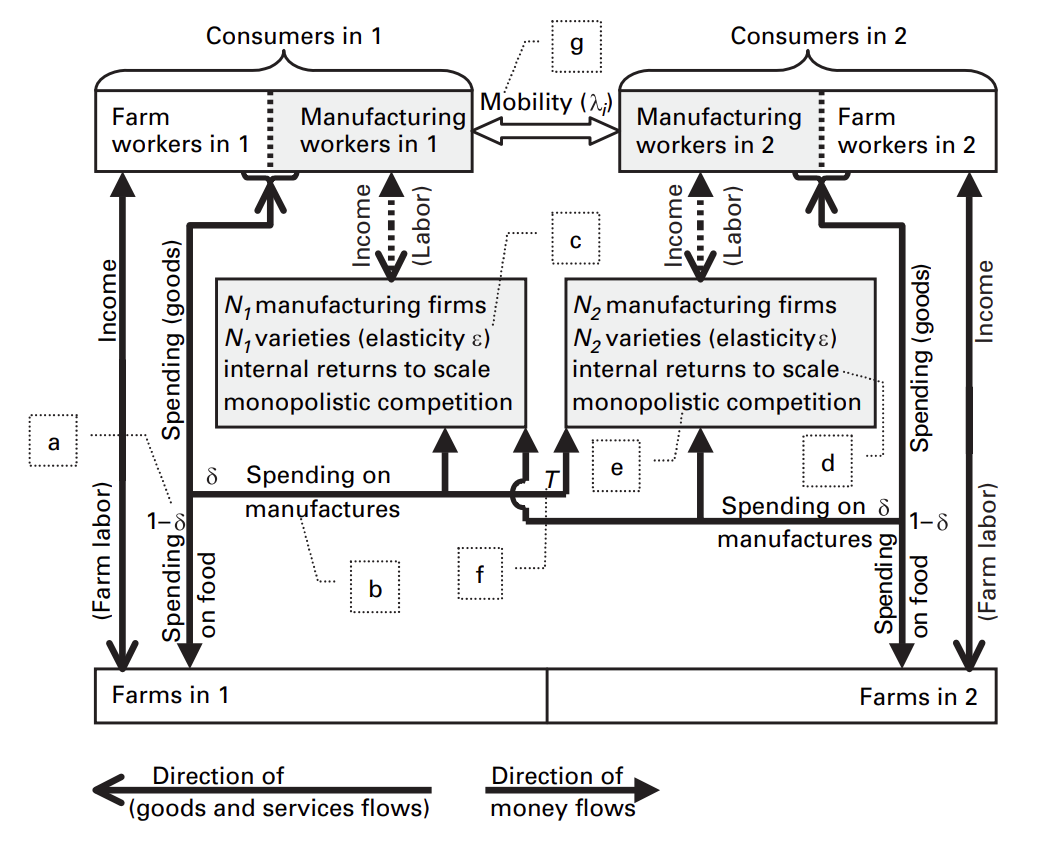
\includegraphics[scale=.3]{./imagen/diag.png}
\end{center}

\nbvspace[3]
\normalsize

LIBRO EN SU SEGUNDA EDICIÓN (Ingles)\\
\large
\nbvspace[1]

\end{center}

\break
\bfseries 

\nbvspace[1]
Título de la obra original:\\
THE NEW INTRODUCTION TO GEOGRAPHICAL ECONOMICS\\
Published in the United States of America by Cambridge University Press, New York\\

\nbvspace[1]

\begin{center}
Sin ninguna revisión de esta obra.\\


\nbvspace[1]
    Propiedad de esta obra:\\ 

    CHRISTIAN LIMBERT PAREDES AGUILERA\\	

    E-mail: soyfode@gmail.com
\end{center}

\nbvspace[1]

Reservados todos los derechos. La reproducción total o parcial de esta obra, por cualquier medio o procedimiento, comprendidos la reprografía y el tratamiento informático, y la distribución de ejemplares de ella mediante alquiler o préstamo públicos, queda rigurosamente prohibida sin la autorización escrita de los titulares del copyright, bajo las sanciones establecidas por las leyes.\\

\center 2022 

\end{titlingpage}


\pagenumbering{roman}

\tableofcontents								%indice

\pagestyle{fancy}
\fancyhead[LE,RO]{\nouppercase{\truncate{0.5\headwidth}{\rightmark}}}
\fancyhead[LO,RE]{\nouppercase{\truncate{0.5\headwidth}{\leftmark}}}



	%---------- Una introducción de econometría 
	    %\chapter{Una introducción a la econometría}

\begin{tcolorbox}[colback=white]
    La \textbf{econometría} se trata de cómo podemos usar la teoría y los datos de la economía, los negocios y las ciencias sociales, junto con las herramientas de las estadísticas, para predecir resultados, responder preguntas del tipo "cuánto" y probar hipótesis.
\end{tcolorbox}

\section{El proceso de investigación}
el proceso de investigación,  generalmente sigue estos pasos:
\begin{enumerate}[\bfseries 1.]
    \item La teoría económica nos da una forma de pensar sobre el problema. ¿Qué variables económicas están involucradas y cuál es la posible dirección de la(s) relación(es)? Todo proyecto de investigación, dada la pregunta inicial, comienza construyendo un modelo económico y enumerando las preguntas (hipótesis) de interés. Surgirán más preguntas durante el proyecto de investigación, pero es bueno enumerar aquellas que te motivan al comienzo del proyecto.
    \item El modelo económico de trabajo conduce a un modelo econométrico. Debemos elegir una forma funcional y hacer algunas suposiciones sobre la naturaleza del término de error.
    \item Se obtienen datos de muestra y se elige un método deseable de análisis estadístico, basado en suposiciones iniciales y una comprensión de cómo se recopilaron los datos.
    \item Las estimaciones de los parámetros desconocidos se obtienen con la ayuda de un paquete de software estadístico, se hacen predicciones y se realizan pruebas de hipótesis.
    \item Se realizan diagnósticos del modelo para comprobar la validez de las suposiciones. Por ejemplo, ¿eran relevantes todas las variables explicativas del lado derecho? ¿Se utilizó una forma funcional adecuada?.
    \item Se analizan y evalúan las consecuencias económicas y las implicaciones de los resultados empíricos. ¿Qué resultados de asignación y distribución de recursos económicos están implícitos y cuáles son sus implicaciones en la elección de políticas? ¿Qué preguntas restantes podrían responderse con más estudios o con datos nuevos y mejores?.
\end{enumerate}

\section{Escribir un artículo de investigación empírica}
\subsection{Escribir una propuesta de investigación}
El resumen debe ser breve, por lo general de no más de 500 palabras, y debe incluir lo siguiente:
\begin{enumerate}[\bfseries 1.]
    \item Una declaración concisa del problema.
    \item Comentarios sobre la información disponible, con una o dos referencias clave.
    \item Una descripción de la investigación diseño que incluye
	\begin{enumerate}[\bfseries a.]
	    \item El modelo económico.
	    \item Los métodos econométricos de estimación e inferencia.
	    \item Fuentes de datos.
	    \item Procedimientos de estimación, prueba de hipótesis y predicción, incluido el software econométrico y la versión utilizada 
	\end{enumerate}
    \item La contribución potencial de la investigación.
\end{enumerate}

\subsection{Un formato para escribir un informe de investigación}
\begin{enumerate}[\bfseries 1.]
    \item \textbf{Declaración del problema}. El lugar para comenzar su informe es con un resumen de las preguntas que desea investigar, así como por qué son importantes y quién debería estar interesado en los resultados. Esta sección introductoria no debe ser técnica y debe motivar al lector a continuar leyendo el artículo. También es útil trazar un mapa del contenido de las siguientes secciones del informe. Esta es la primera sección en la que trabajar y también la última. En el mundo ajetreado de hoy, la atención del lector debe captarse muy rápidamente. Una introducción clara, concisa y bien escrita es imprescindible y posiblemente sea la parte más importante del documento. 
    \item \textbf{Revisión de la literatura}. Resuma brevemente la literatura relevante en el área de investigación que ha elegido y aclare cómo su trabajo amplía nuestro conocimiento. Por todos los medios, cite los trabajos de otros que hayan motivado su investigación, pero sea breve. No tienes que repasar todo lo que se ha escrito sobre el tema. 
    \item \textbf{El modelo económico}. Especifique el modelo económico que utilizó y defina las variables económicas. Indique los supuestos del modelo e identifique las hipótesis que desea probar. Los modelos económicos pueden complicarse. Su tarea es explicar el modelo claramente, pero de la manera más breve y sencilla posible. No utilice jerga técnica innecesaria. Use términos simples en lugar de complicados cuando sea posible. Su objetivo es mostrar la calidad de su pensamiento, no la extensión de su vocabulario. 
    \item \textbf{El modelo econométrico}. Discuta el modelo econométrico que corresponde al modelo económico. Asegúrese de incluir una discusión de las variables en el modelo, la forma funcional, las suposiciones de error y cualquier otra suposición que haga. Utilice una notación lo más simple posible y no abarrote el cuerpo del artículo con largas demostraciones o derivaciones; estos pueden ir en un apéndice técnico. 
    \item \textbf{Los datos}. Describa los datos que utilizó, así como la fuente de los datos y cualquier reserva que tenga sobre su idoneidad. 
    \item \textbf{Los procedimientos de estimación e inferencia}. Describe los métodos de estimación que usaste y por qué los elegiste. Explicar los procedimientos de prueba de hipótesis y su uso. Indique el software utilizado y la versión, como Stata 15 o EViews 10. 
    \item \textbf{Los resultados empíricos y las conclusiones Informe las estimaciones de los parámetros, su interpretación y los valores de las estadísticas de prueba.} Comente su significancia estadística, su relación con estimaciones previas y sus implicaciones económicas. 
    \item \textbf{Posibles extensiones y limitaciones del estudio Su investigación generará preguntas sobre el modelo económico, los datos y las técnicas de estimación.} ¿Qué investigaciones futuras sugieren sus hallazgos y cómo podría llevarlas a cabo? 
    \item \textbf{Agradecimientos}. Es apropiado reconocer a quienes han comentado y contribuido a su investigación. Esto puede incluir a su instructor, un bibliotecario que lo ayudó a encontrar datos o un compañero de estudios que leyó y comentó su trabajo. 
    \item \textbf{Referencias}. Una lista alfabética de la literatura que cita en su estudio, así como referencias a las fuentes de datos que utilizó.
\end{enumerate}

\section{Fuentes de datos económicos}
\begin{itemize}
    \item Resources for Economists (RFE) www.rfe.org
    \item National Bureau of Economic Research (NBER) www.nber.org/data
    \item Economagic https://www.economagic.com/
\end{itemize}


	%---------- El modelo de regresión lineal simple
    	    \chapter{El modelo de regresión lineal simple}


\section{Un modelo econométrico}
Sea $e=$ todo lo demás que afecta a la variable dependiente. Es decir, el termino de error, entonces:
\begin{equation}
    y=\beta_1 + \beta_2 x  + e
\end{equation}

El parámetro desconocido $\beta_2$, la propensión marginal a gastar en alimentos a partir de la renta, nos dice la proporción del aumento de la renta utilizada para la compra de alimentos; responde a la pregunta cuánto ¿Cuánto cambiará el gasto en alimentos dado un cambio en los ingresos, manteniendo todo lo demás constante?.\\
El primer supuesto del modelo de regresión lineal simple es que la relación (2.1) se cumple para los miembros de la población bajo consideración. Afirmamos que la regla de comportamiento $y = \beta_1 + \beta_2 x + e$ se cumple para todos los hogares de la población. Cada semana el gasto en alimentos es igual a $\beta_1$, más una proporción $\beta_2$ de los ingresos, más otros factores, $e$.

\subsection{Proceso de generación de datos}
La selección aleatoria de hogares hace que el primer par de observación $(y_1, x_1)$ sea estadísticamente independiente de todos los demás pares de datos, y cada par de observación $(y_i, x_i)$ es estadísticamente independiente de cualquier otro par de datos, $(y_j, x_j)$, donde $i \neq j$. Suponemos además que las variables aleatorias $y_i$ y $x_i$ tienen una función de densidad de probabilidad conjunta $f(y_i , x_i)$ que describe su distribución de valores. A menudo no conocemos la naturaleza exacta de la distribución conjunta, pero se supone que todos los pares extraídos de la misma población siguen la misma distribución conjunta y, por lo tanto, la de los pares de datos no solo son estadísticamente independientes, sino que también están distribuidos de manera idéntica (iid abreviado o iid). Se dice que los pares de datos que son iid son una muestra aleatoria.\\
Si nuestra primera suposición es cierta, que la regla de comportamiento $y = \beta_1 + \beta_2x + e$ se cumple para todos los hogares de la población, entonces reexpresando (2.1) para cada par de datos $(y_i, x_i)$ tenemos,
$$y_i = \beta_1 + \beta_2 x_i + e_i,\qquad i=1,\ldots, N$$
Esto a veces se denomina proceso de generación de datos (DGP) porque asumimos que los datos observables siguen esta relación.

\subsection{El error aleatorio y la exogeneidad estricta}
El segundo supuesto del modelo de regresión simple (2.1) se refiere al término todo lo demás $e$. Las variables $( y_i , x_i )$ son variables aleatorias porque no sabemos qué valores toman hasta que se elige un hogar en particular y se observan. El término de error $e_i$ también es una variable aleatoria. Todos los demás factores que afectan el gasto en alimentos, excepto los ingresos, serán diferentes para cada hogar de la población, por la única razón de que los gustos y preferencias de todos son diferentes. A diferencia de los gastos e ingresos en alimentos, el término de error aleatorio $e_i$ no es observable; es inobservable. No podemos medir gustos y preferencias de forma directa, como tampoco podemos medir directamente la utilidad económica que se deriva de comer un trozo de tarta. \textbf{El segundo supuesto de regresión es que la variable $x$, el ingreso, no se puede utilizar para predecir el valor de $e_i$}, el efecto de la recopilación de todos los demás factores que afectan el gasto en alimentos por parte del i-ésimo hogar. Dado un valor de ingreso $x_i$ para el i-ésimo hogar, el mejor predictor (óptimo) del error aleatorio $e_i$ es la expectativa condicional, o media condicional, $E ( e_i | x_i )$ . \textbf{La suposición de que $x_i$ no se puede usar para predecir $e_i$ es equivalente a decir que $E ( e_i | x_i ) = 0$}. Es decir, dado el ingreso de un hogar, no podemos hacer nada mejor que predecir que el error aleatorio es cero; los efectos de todos los demás factores sobre el gasto en alimentos promedian, de una manera muy específica, a cero. \\
$E ( e_i | x_i ) = 0$ tiene dos implicaciones. El primero es $E ( e_i | x_i ) = 0 \; \Longrightarrow   E ( e_i) = 0$; si el valor esperado condicional del error aleatorio es cero, entonces la expectativa incondicional del error aleatorio también es cero. En la población, el efecto promedio de todos los factores omitidos resumidos por el término de error aleatorio es cero.\\
La segunda implicación es $E ( e_i | x_i ) = 0 \; \Longrightarrow \; cov( e_i , x_i ) = 0$. Si el valor esperado condicional del error aleatorio es cero, entonces $e_i$, el error aleatorio para la i-ésima observación, tiene covarianza cero y correlación cero, con la correspondiente observación $x_i$. En nuestro ejemplo, el componente aleatorio $e_i$, que representa todos los factores que afectan el gasto en alimentos excepto los ingresos del i-ésimo hogar, no está correlacionado con los ingresos de ese hogar. \textbf{Quizás se pregunte cómo podría demostrarse que eso es cierto. Después de todo, $e_i$ es inobservable. Debe convencerse de que todo lo que podría haberse omitido del modelo no está correlacionado con $x_i$}. La herramienta principal es el razonamiento económico: sus propios experimentos intelectuales (es decir, el pensamiento), la lectura de literatura sobre el tema y las discusiones con colegas o compañeros de clase. Y realmente no podemos probar que $E( e_i | x_i ) = 0$ sea cierto con absoluta certeza en la mayoría de los modelos económicos.\\
Notamos que $E ( e_i | x_i ) = 0$ tiene dos implicaciones. Si alguna de las implicaciones no es verdadera, entonces $E ( e_i | x_i ) = 0$ no es verdadera, es decir,
$$E(e_i|x_i) \neq 0 \; \mbox{si}\; E(e_i)\neq 0\; \mbox{o si}\; cov(e_i,x_i)\neq 0$$
Si $cov ( e_i , x_i ) = 0$, se dice que la variable explicativa $x$ es exógena, siempre que se cumpla nuestra primera suposición de que los pares $(y_i, x_i)$ son iid. Cuando $x$ es exógena, el análisis de regresión se puede utilizar con éxito para estimar $\beta_1$ y $\beta_2$. Para diferenciar la condición más débil $cov ( e_i , x_i ) = 0$, exogeneidad simple, de la condición más fuerte $E ( e_i | x_i ) = 0$, decir que $x$ es estrictamente exógena si $E ( e_i | x_i ) = 0$. Si $cov( e_i , x_i ) \neq  0$, entonces se dice que $x$ es endógena . Cuando $x$ es endógeno, es más difícil, a veces mucho más difícil, realizar una inferencia estadística.

\subsection{La función de regresión}


\end{document}

